\documentclass[12pt,fleqn,a4paper]{article}

\usepackage{latexsym}
\usepackage{url}
\usepackage{xspace}
\usepackage{epsfig}
\usepackage{psfrag}
\usepackage{a4wide}
\usepackage{marvosym}
\usepackage{amsmath,amsfonts,amssymb,amsthm,latexsym}
\usepackage{graphics,graphicx,color,subfigure}
\usepackage{fancyhdr}
\usepackage[english]{babel}
\usepackage[latin1]{inputenc}
% added this package solely because "our" title is way too long and it
% allows to add a line break in the title
%\usepackage[usestackEOL]{stackengine}

\textheight 680pt
\textwidth 460pt
\topmargin -40pt
\oddsidemargin 5pt
\evensidemargin 5pt
\parindent 0pt

\pagestyle{fancyplain} \setlength{\headheight}{16pt}
\renewcommand{\sectionmark}[1]{\markright{\thesection\ #1}}
\lhead[\fancyplain{}{\thepage}]
   {\fancyplain{}{\rightmark}}
\rhead[\fancyplain{}{\leftmark}]
   {\fancyplain{}{\thepage}}
\cfoot{}
\renewcommand{\thesection}{\arabic{section}}
\renewcommand{\thesubsection}{\arabic{section}.\arabic{subsection}}











%definitions for xml-syntax highleiting
\usepackage{listings}

\usepackage{color}
\definecolor{gray}{rgb}{0.4,0.4,0.4}
\definecolor{darkblue}{rgb}{0.0,0.0,0.6}
\definecolor{cyan}{rgb}{0.0,0.6,0.6}

\lstset{
 basicstyle=\ttfamily,
 columns=fullflexible,
 showstringspaces=false,
 commentstyle=\color{gray}\upshape
}

\lstdefinelanguage{XML}
{
 morestring=[b]",
 morestring=[s]{>}{<},
 morecomment=[s]{<?}{?>},
 stringstyle=\color{black},
 identifierstyle=\color{darkblue},
 keywordstyle=\color{cyan},
 morekeywords={xmlns,version,type}% list your attributes here
}
%end of definitions for xml-syntax highleiting













\begin{document}
\begin{titlepage}%Institution
\vspace{2cm}
\centerline{
\large{Department of Computer Sciences}}
\vspace{0.2cm}
\centerline{\large{University of Salzburg}}%Title with one or two Lines(More if wanted)
%\hline
\vspace{2cm}

\centerline{\large{PS Natural Computation}}
\centerline{SS 13/14}
\vspace{1cm}

\centerline{\Large{Design and implementation of a robot task}}
%\centerline{\Large{\bf\Longstack{SIMMA\\Design and implementation of a robot task\\demonstration the effect of
%neuromodulators}} }%Type of the Document
\vspace{1cm}

\vspace{0.4cm}%Date
\centerline{\today}
\vspace{5cm}%Authors

%\hline
\vspace{0.2cm}
Project Members:\\
\centerline{Tobias Auinger, 1220321, auingerto@stud.sbg.ac.at}\\
\centerline{Christian M\"{u}ller, 1123410, mueller110@gmx.net}\\
\centerline{Andreas Pollhammer, 9520061, pollhammerand@stud.sbg.ac.at}\\
\centerline{Stefan Schwarz, 1220024, schwarzst@stud.sbg.ac.at}\\
\vspace {0.8cm}\\

Academic Supervisor: \\
\centerline{Helmut MAYER}
\centerline{helmut@cosy.sbg.ac.at}
\vspace{0.8cm}\\
Correspondence to: \\
\centerline{Universit\"{a}t Salzburg} \\
\centerline{Fachbereich Computerwissenschaften} \\
\centerline{Jakob--Haringer--Stra\ss e 2} \\
\centerline{A--5020 Salzburg} \\
\centerline{Austria}
\clearpage
\end{titlepage}



%%%
%Table of Content
% \setcounter{page}{1}
% \pagenumbering{Roman} %I,II,III... in the TOC
% \tableofcontents

\clearpage
\pagestyle{headings}
\pagenumbering{arabic}  %Better if TOC is variable (more than one page)
\setcounter{page}{1}
\pagenumbering{arabic}  %Better if TOC is variable (more than one page)
\setcounter{page}{1}

\tableofcontents
\newpage

\abstract
{The main goal of this project is designing a task that demonstrates that the usage of neuromodulators can influence the evolution of a neural network in a positive way. For implementation and simulation of the task we use SIMMA "a simulation framework mainly developed for the simulation of mobile autonomous robots and their behaviour".}

%%%
\section{Introduction}
In this class our team of four people designed a task for neural networks.  The main goal was to demonstrate that the usage of neuromodulators can influence the evolution of a neural network in a positive way.

\begin{center}
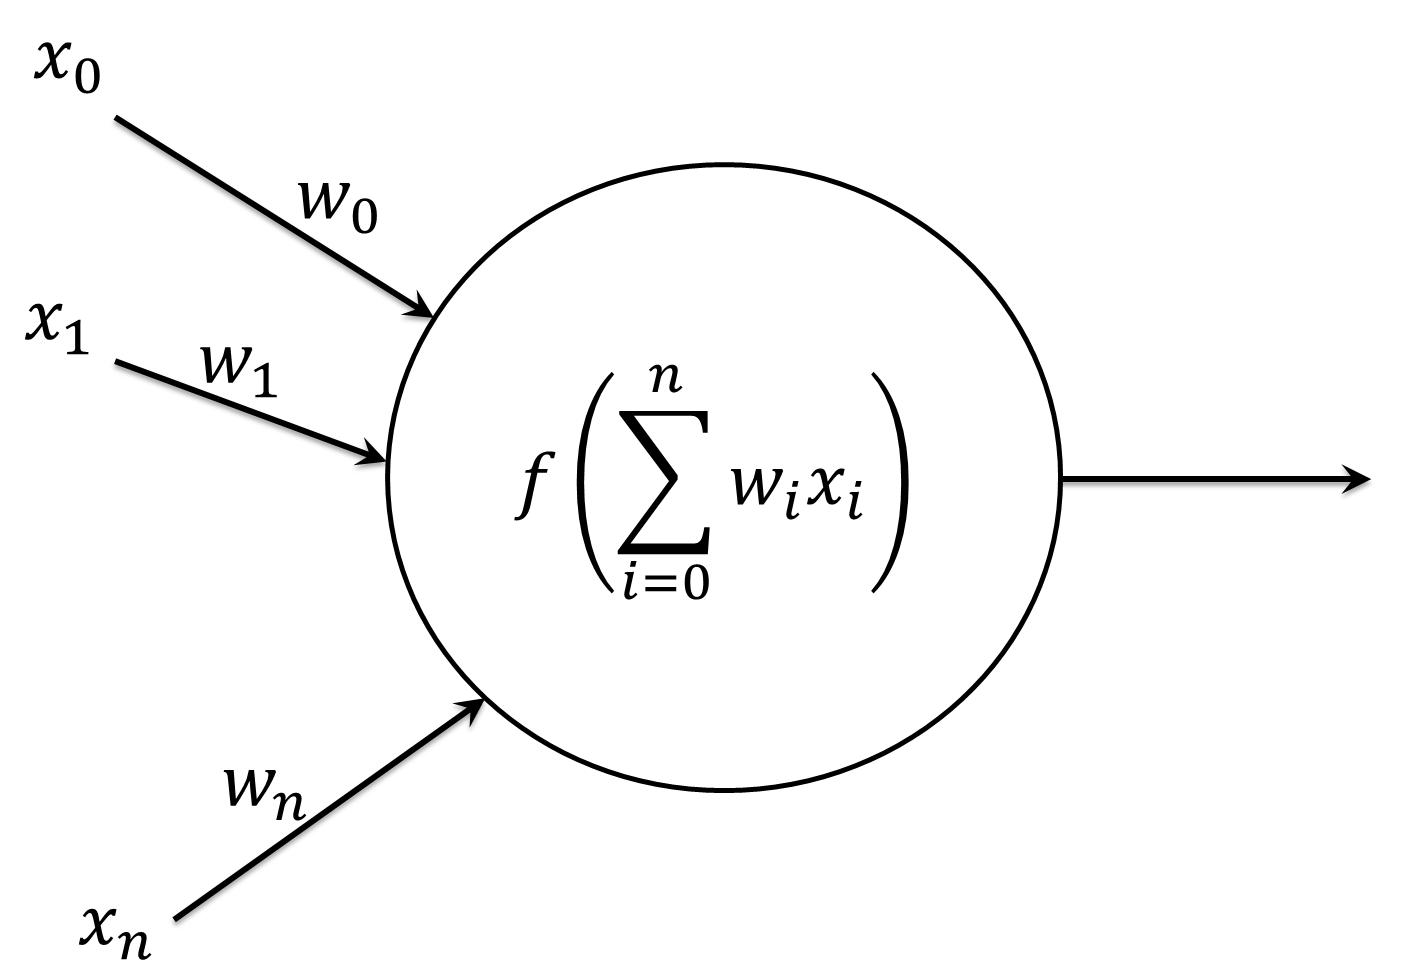
\includegraphics[scale=0.3]{img/neuron.png}
\end{center}


\subsection{SIMMA}

\section{Theoretical Foundation}
\subsection{Neuromodulation}
Neuromodulation basically describes a mechanism, which allows a neuron to switch between different states. There are different approaches how this may work in nature and also how neuromodulators are implemented in different variants of ANNs. In our case the mentioned states of the neuron are associated with a change of bias, the neurons output. In general, it is a complex problem, to find out in which cases bias changes would have a positive effect. So we simply left this to evolution.

For our project, we defined one neuromodulator using the SIMMA class\\ \texttt{simma.ann.modulator.BiasChange}. As Brain we selected the also already existing class \texttt{simma.ann.NeuroModulatorController}. See appendix for a complete listing (xml) of our setup.
In order to get the desired input-output mapping our neural network must be trained.
For that purpose Simma uses evolutionary Algorithms. Evolutionary Algorithms are algorithms that try to implement the principles of darwinian evolution with the purpose of training a neural network. The controller of our robot is such a neural network.
A neural network consists of so called neurons. Each neuron recieves one or more Inputs. The output of is calculated by taking the sum of inputs as an input fot the so called activation function.



\section{The Task}

\subsection{The initial task}
After careful considerations we decided to implement a robot whose task is to collect several pegs, which are randomly distributed within a virtual rectangular world and transport them to a certain place we call spot. While transporting the pegs to the spot the robot has to avoid collisions with one or more enemies following the robot. If the robot is captured by the enemy, it will get some damage, which effects its speed. The robot is supposed to learn this task by means of evolving neural networks. Our hope was that neuromodulators will indeed influence the evolution of our neural network in a positive way. So the neuromodulators assist our robot by learning this task. For implementation and simulation of the task we used SIMMA "a simulation framework mainly developed for the simulation of mobile autonomous robots and their behaviour".

After several tests it turned out, that one part of the task worked very well. Namely the finding and collecting of the pegs, which includes the delivery to the spot. But to our disappointment robots trained to find and collect pegs, seamed to be unable to also learn how to avoid collisions with ghosts. So we focused on the second part of the task, the transportation of pegs through the enemy region.

\subsection{The final task}
For the final task, we divided the region of the simulation in three parts, each with a different purpose. The left side is where the spot spawns, which is the destination for the robots virtual delivery. The right side is the robot's
starting position. Right between those regions, the enemy, named ghost, spawns. This enemy's mere function is to stop the robot's delivery. The ghost does not move around randomly, but it detects the robot's current position for hunting it down, though it has been given a radius in which the robot is followed, which alters the size each new start, depending on the randomly generated number from 0 to 1. This so called "aggression potential" will also influence the robots fitness, given that the bigger this aggression potential is, the harder the robots mission will be. The virtual load carried by the robot does decrease its speed, making it easier to be targeted, since the robot does move slower (or at nearly the same speed, depending on the settings) with a full load than the ghost. Therefore the robot has to drop a certain amount of this load, in order to elude the ghost. By reaching the spot, hence fulfilling its task, the robot will drop the load, or what's left of it, and gains a specific amount of bonus. Does the robot fail its task, whether by getting caught, or not being capable of managing to deliver the load in the given time interval, then it won't have any fitness at all for this round of evaluation. If the ghost's aggression potential is too tiny, dropping a part of the load in order to increase the speed is not necessary, since the robot most likely won't be attacked, thus it should only deposit in need. Thence we thought seeing the effect of neuromodulators in the performing of this task.


\subsection{The Fitness Function}
After putting a lot of thoughts in to the fitness function, we decided to evaluate with the following criteria:
\[ fitness = \frac{\sum_{i=0}^{episodecount} (bonus_i + load_i)*Aggressionpotential_i}{episodecount} \]

If the robot did not manage to reach the spot, the fitness will be 0 for its current episode. 
In contrast to our expectations, prior to the testing of our task, the amount of bonus the robot gets just for reaching the spot is of a fundamental importance. If it is too low the robot will not drop it's pegs. For the individual itself this behaviour may result in death, but the missing survival bonus does not influence the population's fitness significantly. If it is too high the robot drops too many pegs. Some may argue that the above statements are false because of the nature of a bonus. 
The survival bonus is, as its name implies, just a bonus the robot gets on top of its regular performance.


\subsubsection{Considerations on how to improve the robots performance}

When watching the robots movements, it sometimes seams that the robot fails to avoid a collision with the ghost, because there is not enough space within the rectangular world. This happens when the robot tries to gain distance from the ghost while driving against a wall (outer border of the simulated world). We concluded, that this could possibly hinder the robot within its learning process, since there is no way for the robot to even recognize the existence of a wall, besides the fact, that the distance to the ghost does not rise as is should. But the robot could not determine, whether if this is a wall-problem, or the ghost is just faster than the robot. In the former case it should turn around without the need of dropping any pegs. And in the other case it should do just the opposite and drop some pegs. So being aware of this problem, we added the damage-sensor, which we already implemented for our previous task and used it to subtract one damage-point every time the robot collides with the wall. Additionally we added the compass (an existing sensor class in SIMMA) to give the Robot some kind of orientation. By also taking regard of the damage value within the fitness-function, we had been looking forward to evolve a robot which is learning to keep a little distance form the borders of the simulated world. This worked very well as long as we made it easy for the robot to solve the task, meaning a slow moving ghost with only low aggression potential. But with a higher degree of difficulty of the robots task, we were not able to identify any significant improvements. It seemed that the additional sensors just added complexity to the learning process without increasing the level of the reachable fitness. So we returned to our initial keep-it-simple approach.


\section{Components}
To simulate our task we need an area limiting the space, a robot, the delivery destination and an enemy. The limited space is represented by a rectangular area 1.07 meters wide and 0.7 meters in height. The other three components are described in further sections.

\subsection{The Robot}
The circle-shaped robot powered by a battery is our protagonist, which will be evolved to fulfill a certain task. It is able to move around the simulation area using its two wheels. 
%An important factor of the perfomance is the speed. It is influenced by the carried amount of %load, making a fully loaded robot slower and therefore easier to catch.

\begin{center}
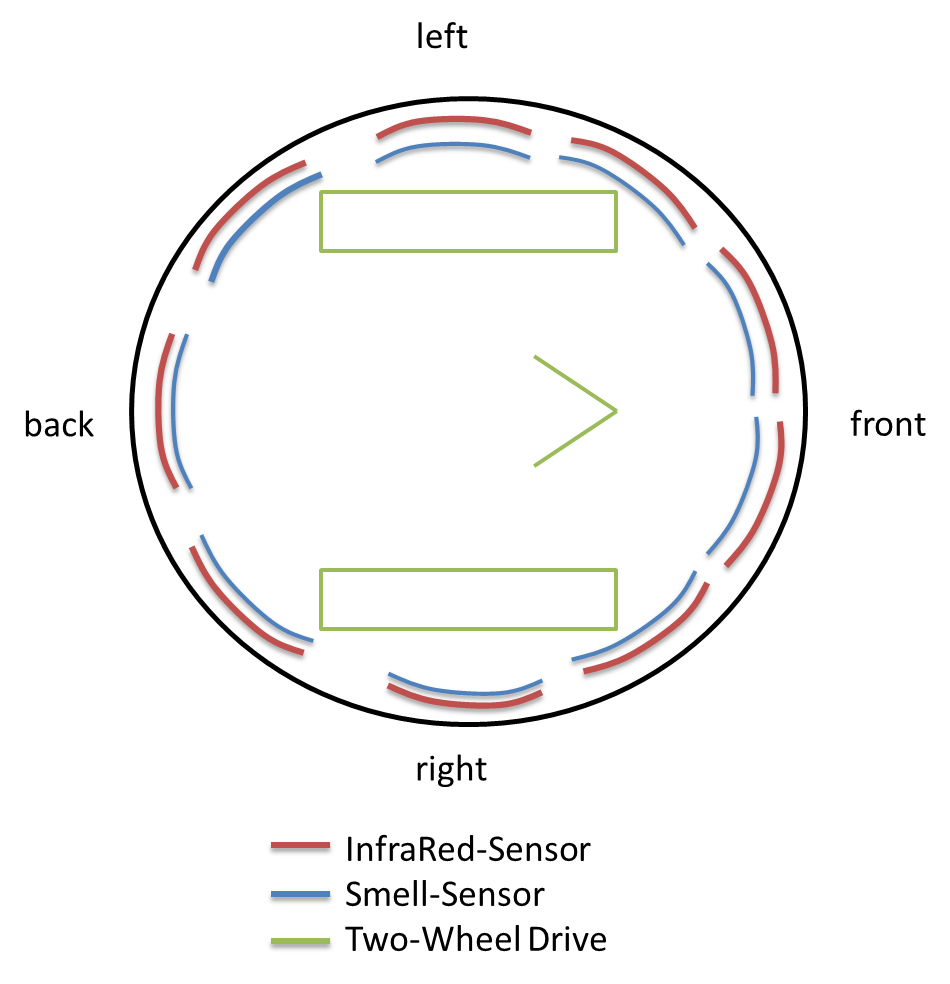
\includegraphics[scale=0.333]{img/robot.png}
\end{center}


\subsubsection{Sensors}
The robot is equipped with the following sensors:
\begin{itemize}
    \item 1 Load-Sensor
    \item 9 Smell-Sensors
    \item 9 Infrared-Sensors
\end{itemize}
The carried load is managed by nine "smell sensors", which are attached around the robot, giving him the ability to see the spot by receiving its produced smell. Determining the distance to the ghost is done by receiving the ghost's emitted heat through nine infrared sensors placed around the robot.

\subsubsection{Damage}
After a collision has been detected between the ghost and the robot, the robot is harmed, the robot's capability of movement is declined and therefore the robot failed its task, resulting in a fitness of 0.

\subsubsection{Actuator}


\subsection{The Enemy}
%
\includegraphics[scale=0.5]{img/ghost.png}

The Enemy, called ghost is represented in SIMMA by a white circle. We therfore implemented a class called \texttt{Ghost} for which the following settings can be made in the configuration-file: The speed of the ghost can be set by a tag called \texttt{Speed} with properties \texttt{VX} and \texttt{VY} for the speed in direction of the x-axis or y-axis resepctively. The settings for \texttt{MoveArea} were intended to capture the ghost within a given aria, but are not used at current.

\subsection{The Spot}
The spot, being the delivery destination, is emitting smell in every direction of the simulation space, making it recognizeable and distinguishable from the ghost. It also serves the purpose as a safe zone for the robot.

\section{Results}
For the results we evolved two robots, distuingished by the usage of neuromodulators and therefore a different brain. Despite of that, everything had to be equivalent for the comparision of those robots.

\subsection{Evolution}
asdf

\subsection{Performance}
asf

\section{Conclusion}
By evolving and comparing the two robots with our implemented task we noticed a positive influence not only in performance, but also in the evolution.

\newpage
% links go here, NOT in references
%%%
\section{Links}

\begin{itemize}
\item Project Page: \url{http://student.cosy.sbg.ac.at/~cmueller/natcomp/}
\item PS Page: \url{http://www.cosy.sbg.ac.at/~helmut/Teaching/NaturalComputation/proseminar.html}
\end{itemize}

\bibliography{}  % .bib files here



\section{Appendix}

\subsection{XML-Listing}

\lstset{language=XML}
\begin{lstlisting}
<Configuration Name="Peg Pushing Evolution">
<General>
 <UpdateXMLFile>false</UpdateXMLFile>
 <SimTimeStep>0.1</SimTimeStep>
 <ScreenScale>904.0</ScreenScale>
 <ScreenRefreshTime>0.1</ScreenRefreshTime>
 <Animate3D>true</Animate3D>
</General>
<Experiment>
 <Objects>
  <World Name="World">
   <Class>simma.worlds.RectangularArena</Class>
   <Width>1.05</Width>
   <Height>0.7</Height>
   <Depth>0.3</Depth>
  </World>
  <Robot Name="Rescuer">
   <Class>simma.robots.CircleRobot</Class>
   <BoundingRadius>0.03</BoundingRadius>
   <MotionTrail>false</MotionTrail>
   <ResetMode>None</ResetMode>
   <Height>0.15</Height>
   <Controller Name="Brain">
    <Class>simma.ann.NeuroModulatorController</Class>
    <!--<Class>simma.ann.NeuroFeedForwardController</Class>-->
    <Structure>20-20-3</Structure>
    <LearnRate>0.01</LearnRate>
    <MaxDose>1.0</MaxDose>
    <ResetMode>None</ResetMode>
    <Areas>1</Areas>
   
    <Modulator Name="ModA">
     <Color>GREEN</Color>
    </Modulator>
    <Reaction>
     <Class>simma.ann.modulator.BiasChange</Class>
     <Positive>true</Positive>
    </Reaction>
    <Evolution Enabled="true">
     <Neurons>false</Neurons>
     <Links>true</Links>
     <Weights>true</Weights>
     <MutationRate>0.0050</MutationRate>
     <CrossoverPoints>2</CrossoverPoints>
     <OutputBias>true</OutputBias>
    </Evolution>
   </Controller>
   <Actuator Name="Two-Wheel Drive">
    <Class>simma.kernel.equipment.TwoWheelDrive</Class>
    <Mass>0.15</Mass>
    <Gain>5.0</Gain>
    <Offset>-0.5</Offset>
    <MotorResistance>2.5</MotorResistance>
    <AxisLength>0.03</AxisLength>
    <WheelRadius>0.01</WheelRadius>
    <Position>
     <R>0.0</R>
     <Phi>0.0</Phi>
    </Position>
   </Actuator>
   <Sensor Name="LoadSensor">
    <Class>simma.equipment.sensors.LoadSensor</Class>
    <Position>
     <R>0.030</R>
     <Phi>-40.0</Phi>
    </Position>
    <GroundClearance>0.001</GroundClearance>
    <Mass>0.0020</Mass>
   </Sensor>
   <Sensor Name="DamageSensor">
    <Class>simma.equipment.sensors.DamageSensor</Class>
    <Position>
     <R>0.030</R>
     <Phi>-40.0</Phi>
    </Position>
    <GroundClearance>0.001</GroundClearance>
    <Mass>0.0020</Mass>
   </Sensor>
   <Sensor Name="InfraRedLeftBehind">
    <Class>simma.equipment.sensors.InfraRedSensor</Class>
    <Position>
     <R>0.025</R>
     <Phi>-135.0</Phi>
    </Position>
    <GroundClearance>0.015</GroundClearance>
    <Mass>0.0020</Mass>
   </Sensor>
   <Sensor Name="InfraRedLeft">
    <Class>simma.equipment.sensors.InfraRedSensor</Class>
    <Position>
     <R>0.025</R>
     <Phi>-90.0</Phi>
    </Position>
    <GroundClearance>0.015</GroundClearance>
    <Mass>0.0020</Mass>
   </Sensor>
   <Sensor Name="InfraRedHalfLeft">
    <Class>simma.equipment.sensors.InfraRedSensor</Class>
    <Position>
     <R>0.025</R>
     <Phi>-45.0</Phi>
    </Position>
    <GroundClearance>0.015</GroundClearance>
    <Mass>0.0020</Mass>
   </Sensor>
   <Sensor Name="InfraRedCenterLeft">
    <Class>simma.equipment.sensors.InfraRedSensor</Class>
    <Position>
     <R>0.025</R>
     <Phi>-15.0</Phi>
    </Position>
    <GroundClearance>0.015</GroundClearance>
    <Mass>0.0020</Mass>
   </Sensor>
   <Sensor Name="InfraRedCenterRight">
    <Class>simma.equipment.sensors.InfraRedSensor</Class>
    <Position>
     <R>0.025</R>
     <Phi>15.0</Phi>
    </Position>
    <GroundClearance>0.015</GroundClearance>
    <Mass>0.0020</Mass>
   </Sensor>
   <Sensor Name="InfraRedHalfRight">
    <Class>simma.equipment.sensors.InfraRedSensor</Class>
    <Position>
     <R>0.025</R>
     <Phi>45.0</Phi>
    </Position>
    <GroundClearance>0.015</GroundClearance>
    <Mass>0.0020</Mass>
   </Sensor>
   <Sensor Name="InfraRedRight">
    <Class>simma.equipment.sensors.InfraRedSensor</Class>
    <Position>
     <R>0.025</R>
     <Phi>90.0</Phi>
    </Position>
    <GroundClearance>0.015</GroundClearance>
    <Mass>0.0020</Mass>
   </Sensor>
   <Sensor Name="InfraRedRightBehind">
    <Class>simma.equipment.sensors.InfraRedSensor</Class>
    <Position>
     <R>0.025</R>
     <Phi>135.0</Phi>
    </Position>
    <GroundClearance>0.015</GroundClearance>
    <Mass>0.0020</Mass>
   </Sensor>
   <Sensor Name="InfraRedBehind">
    <Class>simma.equipment.sensors.InfraRedSensor</Class>
    <Position>
     <R>0.025</R>
     <Phi>180.0</Phi>
    </Position>
    <GroundClearance>0.015</GroundClearance>
    <Mass>0.0020</Mass>
   </Sensor>
   <Sensor Name="SmellLeftBehind">
    <Class>simma.equipment.sensors.SmellSensor</Class>
    <Position>
     <R>0.025</R>
     <Phi>-135.0</Phi>
    </Position>
    <GroundClearance>0.015</GroundClearance>
    <Mass>0.0020</Mass>
    <Substance>Smell</Substance>
   </Sensor>
   <Sensor Name="SmellLeft">
    <Class>simma.equipment.sensors.SmellSensor</Class>
    <Position>
     <R>0.025</R>
     <Phi>-90.0</Phi>
    </Position>
    <GroundClearance>0.015</GroundClearance>
    <Mass>0.0020</Mass>
    <Substance>Smell</Substance>
   </Sensor>
   <Sensor Name="SmellHalfLeft">
    <Class>simma.equipment.sensors.SmellSensor</Class>
    <Position>
     <R>0.025</R>
     <Phi>-45.0</Phi>
    </Position>
    <GroundClearance>0.015</GroundClearance>
    <Mass>0.0020</Mass>
    <Substance>Smell</Substance>
   </Sensor>
   <Sensor Name="SmellCenterLeft">
    <Class>simma.equipment.sensors.SmellSensor</Class>
    <Position>
     <R>0.025</R>
     <Phi>-15.0</Phi>
    </Position>
    <GroundClearance>0.015</GroundClearance>
    <Mass>0.0020</Mass>
    <Substance>Smell</Substance>
   </Sensor>
   <Sensor Name="SmellCenterRight">
    <Class>simma.equipment.sensors.SmellSensor</Class>
    <Position>
     <R>0.025</R>
     <Phi>15.0</Phi>
    </Position>
    <GroundClearance>0.015</GroundClearance>
    <Mass>0.0020</Mass>
    <Substance>Smell</Substance>
   </Sensor>
   <Sensor Name="SmellHalfRight">
    <Class>simma.equipment.sensors.SmellSensor</Class>
    <Position>
     <R>0.025</R>
     <Phi>45.0</Phi>
    </Position>
    <GroundClearance>0.015</GroundClearance>
    <Mass>0.0020</Mass>
    <Substance>Smell</Substance>
   </Sensor>
   <Sensor Name="SmellRight">
    <Class>simma.equipment.sensors.SmellSensor</Class>
    <Position>
     <R>0.025</R>
     <Phi>90.0</Phi>
    </Position>
    <GroundClearance>0.015</GroundClearance>
    <Mass>0.0020</Mass>
    <Substance>Smell</Substance>
   </Sensor>
   <Sensor Name="SmellRedRightBehind">
    <Class>simma.equipment.sensors.SmellSensor</Class>
    <Position>
     <R>0.025</R>
     <Phi>135.0</Phi>
    </Position>
    <GroundClearance>0.015</GroundClearance>
    <Mass>0.0020</Mass>
    <Substance>Smell</Substance>
   </Sensor>
   <Sensor Name="SmellBehind">
    <Class>simma.equipment.sensors.SmellSensor</Class>
    <Position>
     <R>0.025</R>
     <Phi>180.0</Phi>
    </Position>
    <GroundClearance>0.015</GroundClearance>
    <Mass>0.0020</Mass>
    <Substance>Smell</Substance>
   </Sensor><!--<Sensor Name="LightLeft"> <Class>simma.equipment.sensors.ParticleSensor</Class>
    <Position> <R>0.015</R> <Phi>-90.0</Phi> </Position> <GroundClearance>0.06</GroundClearance>
    <Mass>0.0020</Mass> <Substance>Photon</Substance> <ApertureAngle>90.0</ApertureAngle>
    </Sensor> <Sensor Name="LightCenter"> <Class>simma.equipment.sensors.ParticleSensor</Class>
    <Position> <R>0.0175</R> <Phi>0.0</Phi> </Position> <GroundClearance>0.045</GroundClearance>
    <Mass>0.0020</Mass> <Substance>Photon</Substance> <ApertureAngle>90.0</ApertureAngle>
    </Sensor> <Sensor Name="LightRight"> <Class>simma.equipment.sensors.ParticleSensor</Class>
    <Position> <R>0.015</R> <Phi>90.0</Phi> </Position> <GroundClearance>0.06</GroundClearance>
    <Mass>0.0020</Mass> <Substance>Photon</Substance> <ApertureAngle>90.0</ApertureAngle>
    </Sensor> -->
   <Mass>0.2</Mass>
  </Robot><!-- <Peg Name="LostPeg"> <Class>simma.equipment.LostPeg</Class>
   <Particle Name="Heat"> <Quantum>1.0</Quantum> <Color>BLUE</Color> </Particle>
   <BoundingRadius>0.02</BoundingRadius> <Height>0.015</Height> <Color>RED</Color>
   <ResetMode>Random</ResetMode> <MotionTrail>true</MotionTrail> </Peg> <Peg
   Name="LostPeg"> <Class>simma.equipment.LostPeg</Class> <Particle Name="Heat">
   <Quantum>1.0</Quantum> <Color>BLUE</Color> </Particle> <BoundingRadius>0.02</BoundingRadius>
   <Height>0.015</Height> <Color>RED</Color> <ResetMode>Random</ResetMode> <MotionTrail>true</MotionTrail>
   </Peg> <Peg Name="LostPeg"> <Class>simma.equipment.LostPeg</Class> <Particle
   Name="Heat"> <Quantum>1.0</Quantum> <Color>BLUE</Color> </Particle> <BoundingRadius>0.02</BoundingRadius>
   <Height>0.015</Height> <Color>RED</Color> <ResetMode>Random</ResetMode> <MotionTrail>true</MotionTrail>
   </Peg> --><!--<Peg Name="LostPeg"> <Class>simma.equipment.LostPeg</Class>
   <Particle Name="Heat"> <Quantum>1.0</Quantum> <Color>WHITE</Color> </Particle>
   <BoundingRadius>0.02</BoundingRadius> <Height>0.015</Height> <Color>RED</Color>
   <ResetMode>Random</ResetMode> <MotionTrail>true</MotionTrail> </Peg> <Peg
   Name="LostPeg"> <Class>simma.equipment.LostPeg</Class> <Particle Name="Heat">
   <Quantum>1.0</Quantum> <Color>WHITE</Color> </Particle> <BoundingRadius>0.02</BoundingRadius>
   <Height>0.015</Height> <Color>RED</Color> <ResetMode>Random</ResetMode> <MotionTrail>true</MotionTrail>
   </Peg> <Peg Name="LostPeg"> <Class>simma.equipment.LostPeg</Class> <Particle
   Name="Heat"> <Quantum>1.0</Quantum> <Color>WHITE</Color> </Particle> <BoundingRadius>0.02</BoundingRadius>
   <Height>0.015</Height> <Color>RED</Color> <ResetMode>Random</ResetMode> <MotionTrail>true</MotionTrail>
   </Peg> <Peg Name="LostPeg"> <Class>simma.equipment.LostPeg</Class> <Particle
   Name="Heat"> <Quantum>1.0</Quantum> <Color>WHITE</Color> </Particle> <BoundingRadius>0.02</BoundingRadius>
   <Height>0.015</Height> <Color>RED</Color> <ResetMode>Random</ResetMode> <MotionTrail>true</MotionTrail>
   </Peg> <Peg Name="LostPeg"> <Class>simma.equipment.LostPeg</Class> <Particle
   Name="Heat"> <Quantum>1.0</Quantum> <Color>WHITE</Color> </Particle> <BoundingRadius>0.02</BoundingRadius>
   <Height>0.015</Height> <Color>RED</Color> <ResetMode>Random</ResetMode> <MotionTrail>true</MotionTrail>
   </Peg> <Peg Name="LostPeg"> <Class>simma.equipment.LostPeg</Class> <Particle
   Name="Heat"> <Quantum>1.0</Quantum> <Color>WHITE</Color> </Particle> <BoundingRadius>0.02</BoundingRadius>
   <Height>0.015</Height> <Color>RED</Color> <ResetMode>Random</ResetMode> <MotionTrail>true</MotionTrail>
   </Peg> <Peg Name="LostPeg"> <Class>simma.equipment.LostPeg</Class> <Particle
   Name="Heat"> <Quantum>1.0</Quantum> <Color>WHITE</Color> </Particle> <BoundingRadius>0.02</BoundingRadius>
   <Height>0.015</Height> <Color>RED</Color> <ResetMode>Random</ResetMode> <MotionTrail>true</MotionTrail>
   </Peg> -->
  <Ghost Name="Ghost">
   <Class>simma.equipment.Ghost</Class>
   <Particle Name="Heat">
    <Quantum>1.0</Quantum>
    <Color>WHITE</Color>
   </Particle>
   <BoundingRadius>0.045</BoundingRadius>
   <Height>0.015</Height>
   <Color>WHITE</Color>
   <ResetMode>Random</ResetMode>
   <MotionTrail>false</MotionTrail>
   <MoveArea>
    <X>0.1</X>
    <Y>0.1</Y>
    <XX>0.98</XX>
    <YY>0.67</YY>
   </MoveArea>
   <Speed>
    <VX>0.0095</VX>
    <VY>0.0095</VY>
   </Speed>
  </Ghost><!--<Ghost Name="Ghost"> <Class>simma.equipment.Ghost</Class>
   <Particle Name="Smell"> <Quantum>1.0</Quantum> <Color>WHITE</Color> </Particle>
   <BoundingRadius>0.05</BoundingRadius> <Height>0.015</Height> <Color>WHITE</Color>
   <ResetMode>Random</ResetMode> <MotionTrail>false</MotionTrail> <MoveArea>
   <X>0.3</X> <Y>0.1</Y> <XX>0.98</XX> <YY>0.67</YY> </MoveArea> <Speed> <VX>0.001</VX>
   <VY>0.001</VY> </Speed> </Ghost> <Ghost Name="Ghost"> <Class>simma.equipment.Ghost</Class>
   <Particle Name="Smell"> <Quantum>1.0</Quantum> <Color>WHITE</Color> </Particle>
   <BoundingRadius>0.05</BoundingRadius> <Height>0.015</Height> <Color>WHITE</Color>
   <ResetMode>Random</ResetMode> <MotionTrail>false</MotionTrail> <MoveArea>
   <X>0.01</X> <Y>0.01</Y> <XX>0.98</XX> <YY>0.67</YY> </MoveArea> <Speed> <VX>0.00</VX>
   <VY>0.01</VY> </Speed> </Ghost> -->
  <Spot Name="Spot">
   <Class>simma.equipment.Spot</Class>
   <Particle Name="Smell">
    <Quantum>1.0</Quantum>
    <Color>YELLOW</Color>
   </Particle>
   <BoundingRadius>0.06</BoundingRadius>
   <Color>yellow</Color>
   <ResetMode>None</ResetMode>
  </Spot>
 </Objects>
 <Reporter Name="RescueTaskReporter">
  <Class>simma.reporters.RescueTaskReporter</Class>
  <ReportObject>Rescuer</ReportObject>
  <EpisodeCount>50</EpisodeCount>
  <TestPhase>false</TestPhase>
  <ReportTimeInterval>800.0</ReportTimeInterval>
 </Reporter>
</Experiment>
<Evolution>
 <Runs>1</Runs>
 <PopulationSize>20</PopulationSize>
 <MinimalGenerations>10</MinimalGenerations>
 <MaximalGenerations>600</MaximalGenerations>
 <FitnessThreshold>300000.0</FitnessThreshold>
</Evolution>
</Configuration>
\end{lstlisting}

%
% end of document
%
\end{document}


